\documentclass[border=10pt]{standalone}
\usepackage{tikz}
\usetikzlibrary{arrows.meta, shapes, calc}

\begin{document}
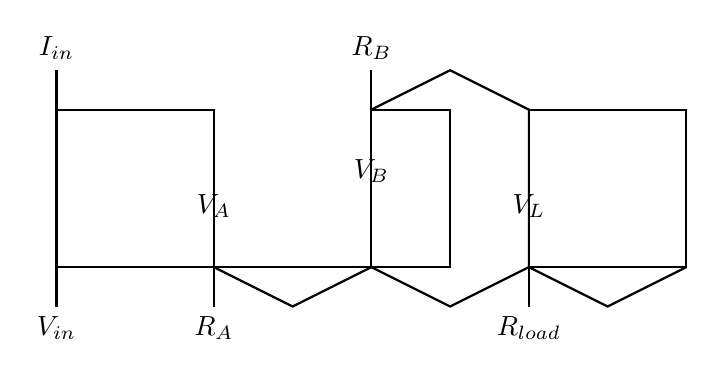
\begin{tikzpicture}[>=Stealth, thick]

% Voltage source
\draw (0,0) -- (2,0) coordinate (A);
\draw (0,0) -- (0,2) -- (2,2) -- (2,0);
\draw (0,0) -- (0,-0.5) node[below] {$V_{in}$};
\draw (0,2) -- (0,2.5) node[above] {$I_{in}$};

% Resistor RA
\draw (2,0) -- (4,0) coordinate (B);
\draw (2,0) -- (3,-0.5) -- (4,0);
\draw (2,0) -- (2,-0.5) node[below] {$R_A$};
\draw (2,0) -- (2,0.5) node[above] {$V_A$};

% Node connections
\draw (4,0) -- (4,2) coordinate (C);
\draw (4,0) -- (5,-0.5) -- (6,0) -- (6,2) -- (5,2.5) -- (4,2);

% Resistor RB
\draw (4,2) -- (5,2) -- (5,0) -- (4,0);
\draw (4,2) -- (4,2.5) node[above] {$R_B$};
\draw (4,2) -- (4,1.5) node[below] {$V_B$};

% Load Resistor R_load
\draw (6,0) -- (8,0) -- (8,2) -- (6,2);
\draw (6,0) -- (7,-0.5) -- (8,0);
\draw (6,0) -- (6,-0.5) node[below] {$R_{load}$};
\draw (6,0) -- (6,0.5) node[above] {$V_L$};

\end{tikzpicture}
\end{document}